\documentclass[UTF8,a4paper,10pt,nocolorlinks]{ctexart}
\usepackage[left=2.50cm, right=2.50cm, top=2.50cm, bottom=2.50cm]{geometry} %页边距
\CTEXsetup[format={\Large\bfseries}]{section} %设置章标题居左   
\usepackage{ctex}
\CTEXoptions[today=old]
\usepackage{cite}
% 代码块儿
\usepackage{textcomp} % 必须加上,否则报错
\usepackage{listings}
\usepackage{xcolor}
% \usepackage{fontspec}
% \setmonofont{Consolas}
\usepackage{varioref}       % ref 跨页调用
\usepackage{ctex}
\usepackage{multicol}
\usepackage{amssymb}        % 等于号 上面 加一个三角形
\usepackage{setspace}
\usepackage{tikz} % package used for the tikz
\usepackage{mdframed}
\usepackage{titletoc}
\usepackage{etoolbox}

\usepackage{helvet}
\usepackage{caption}
\usepackage{multicol} %用于实现在同一页中实现不同的分栏
\usepackage{changepage}
\usepackage{graphics}
\usepackage{amsmath, amsfonts, amssymb} % math equations, symbols
\usepackage[english]{babel}
\usepackage{color}      % color content
\usepackage{graphicx}   % import figures
\usepackage{url}        % hyperlinks
\usepackage{bm}         % bold type for equations
\usepackage{multirow}
\usepackage{booktabs}
\usepackage{epstopdf}
\usepackage{epsfig}
\usepackage{algorithm}
\usepackage{algorithmic}

\usepackage[pagestyles]{titlesec}
% \renewcommand{\algorithmicrequire}{ \textbf{Input:}}     % use Input in the format of Algorithm  
% \renewcommand{\algorithmicinput}{ \textbf{Input:}}     % use Input in the format of Algorithm  
\renewcommand{\algorithmicensure}{ \textbf{Input:}} % use Initialize in the format of Algorithm  
% \renewcommand{\algorithmicreturn}{ \textbf{Output:}}     % use Output in the format of Algorithm  
\renewcommand{\figurename}{图}
% 引用参考文献标号显示在右上角
\newcommand{\upcite}[1]{\textsuperscript{\textsuperscript{\cite{#1}}}}

\newpagestyle{teststyle}{
  \sethead{学号: 2019520941}{\sectiontitle}{第\thepage页}
  \renewcommand{\makeheadrule}{
    \makebox[0pt][l]{\rule[-.3\baselineskip]{\linewidth}{.5pt}}
    \rule[-.4\baselineskip]{\linewidth}{.5pt}
  }
}
\usepackage{color}
\usepackage{subfigure}
\usepackage{changepage}
\usepackage{fancyhdr} %设置页眉、页脚
\pagestyle{fancy}  %%%单线页眉
\fancyhead{}
\fancyhead[LO]{学习总结}
\fancyhead[RO]{冯学伟}
% \fancyfoot[RO]{\thepage}
\fancypagestyle{plain}{%
  \pagestyle{fancy}
}
\usepackage{shorttoc}
\usepackage{xcolor}
\usepackage{mdframed}
\usepackage{titletoc}
% \renewcommand{\today}{\CJKnumber\year 年 \CJKnumber\month 月 \CJKnumber\day 日}

\DeclareRobustCommand{\chuhao}{\fontsize{42pt}{\baselineskip}\selectfont}  % 初号
\DeclareRobustCommand{\xiaochu}{\fontsize{36pt}{\baselineskip}\selectfont} % 小初
\DeclareRobustCommand{\yihao}{\fontsize{26pt}{\baselineskip}\selectfont}   % 一号
\DeclareRobustCommand{\xiaoyi}{\fontsize{24pt}{\baselineskip}\selectfont}  % 小一
\DeclareRobustCommand{\erhao}{\fontsize{22pt}{\baselineskip}\selectfont}   % 二号
\DeclareRobustCommand{\xiaoer}{\fontsize{18pt}{\baselineskip}\selectfont}  % 小二
\DeclareRobustCommand{\sanhao}{\fontsize{16pt}{\baselineskip}\selectfont}  % 三号 
\DeclareRobustCommand{\xiaosan}{\fontsize{15pt}{\baselineskip}\selectfont} % 小三
\DeclareRobustCommand{\sihao}{\fontsize{14pt}{\baselineskip}\selectfont}   % 四号
\DeclareRobustCommand{\xiaosi}{\fontsize{12pt}{\baselineskip}\selectfont}  % 小四
\DeclareRobustCommand{\wuhao}{\fontsize{10.5pt}{\baselineskip}\selectfont} % 五号
\DeclareRobustCommand{\xiaowu}{\fontsize{9pt}{\baselineskip}\selectfont}   % 小五
\DeclareRobustCommand{\liuhao}{\fontsize{7.5pt}{\baselineskip}\selectfont} % 六号
\DeclareRobustCommand{\xiaoliu}{\fontsize{6.5pt}{\baselineskip}\selectfont}% 小六
\DeclareRobustCommand{\qihao}{\fontsize{5.5pt}{\baselineskip}\selectfont}  % 七号

\lstset{numbers=left,numberstyle=\tiny,
breaklines=true,  %代码过长则换行
keywordstyle=\color{blue!70},commentstyle=\color{red!50!green!50!blue!50},frame=shadowbox, rulesepcolor=\color{gray!20!green!20!blue!20},escapeinside=``,xleftmargin=2em,xrightmargin=2em, aboveskip=1em}

\providecommand{\keywords}[1]{\textbf{\textit{keywords---}} #1}

 
\usepackage{hyperref} %bookmarks
% \usepackage[colorlinks,linkcolor=red,anchorcolor=blue,citecolor=green,CJKbookmarks=True]{hyperref}
\hypersetup{colorlinks, bookmarks, unicode} % unicode
 
\captionsetup[figure]{labelfont={bf},labelformat={default},labelsep=period,name={图}}
\newenvironment{figurehere}
{\def\@captype{figure}}
{}

\title{
    \huge{\textbf{2020.07.07 第一次总结}}\\
}
\author{冯学伟}
\date{2020.07.07}

\begin{document}
    \maketitle
    % \renewcommand{\contentsname}{目录}  % 将Contents改为目录
    % \tableofcontents
    % \thispagestyle{empty} % 设置当前页 页版式
    
   
    本周计划: 
    \begin{itemize}
      \item 理论学习: 继续就那本书进行学习, 按照进度, 应该可以看一章多一点.
      \item 调bug: 将HITL调通
    \end{itemize}
    % \section{本周的学习总结}
    %     \subsection{chapter 3}
    %     本章, 主要介绍了刚体运动的运动学(kinematics)和动力学(dynamics); 其中主要定义了
    %     \begin{itemize}
    %       \item 位置和速度的关系(kinematics)
    %       \item 动力学表达式
    %       \item 12个状态量的表达式
    %     \end{itemize}
    %     首先介绍了\textcolor{red}{声明了MAV状态变量}, 12个, 
    %     其中, 和平移运动相关的三个位置变量(ned), 
    %     三个速度变量($u, v, \omega$, $i^{b}, j^{b}, k^{b}$), 
    %     三个角度(roll($F^{v2}$), pitch($F^{v1}$), yaw($F^{v}$)), 
    %     三个角速度($i^{b}, j^{b}, k^{b}$); 
    %     其次推导了\textcolor{red}{运动学, 即位置和速度的关系}, 
    %     我们需要将其从位置的导数即速度从体坐标系下转换到vehicle坐标系下进行计算.  
    %     因为位置是NED, 属于惯性坐标系下的值, 那么速度也是表示在惯性坐标系, 而惯性坐标系和vehicle坐标系三轴的指向是一样的, 唯一不一样的是二者的原点位置不同, 前者的原点位置是在地心, 后者是在MAV的质心, 且从体坐标系到vehicle存在确定的旋转矩阵, 故我们需要做这样的一个变换, 从而使其统一化;
    %     最后也推导了\textcolor{red}{动力学方程}, 针对牛顿第二定律的应用, 分别介绍了其在MAV的平移运动和旋转运动的动力学模型,
    %     \subsection{chapter 4}
    %     本章, 主要关注于力和力矩的梳理, 主要的来源是
    %     \begin{itemize}
    %       \item 重力(没有产生力矩)
    %       \item 空气动力($f_{a}, m_{a}$)
    %       \item 推力($f_{p}, m_{p}$)
    %       \item 大气的扰动, 即风速
    %     \end{itemize}
    %     关于重力, 推导出了其与欧拉角的数学关系式; 关于空气动力, 从纵向和横向两个方面进行了描述, 其中也介绍了无人机的控制平面, 包括 方向舵-副翼-升降舵无人机架构; 方向升降舵无人机架构; 升降翼舵无人机架构, 以及后二者和前者的转化关系式. 
    % \clearpage
    % \section{代码框架的梳理}
    %     结合框图来进行阐述
      
    % \clearpage
    % \section{simulation}
    % \begin{figure}[htbp]
    %   \centering
    %   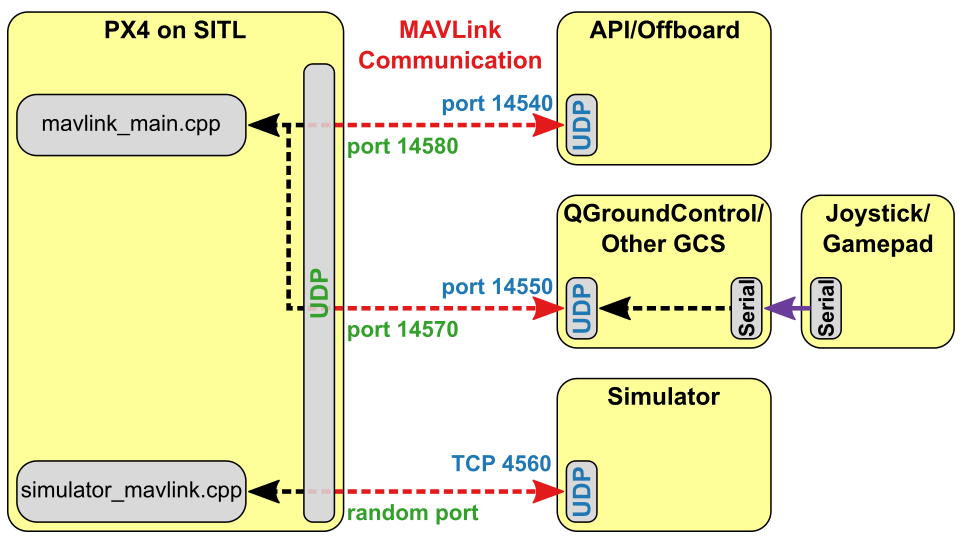
\includegraphics[width=0.8\textwidth]{picture/sitl.png}
    %   \caption{SITL}
    % \end{figure}
    % \begin{figure}[htbp]
    %   \centering
    %   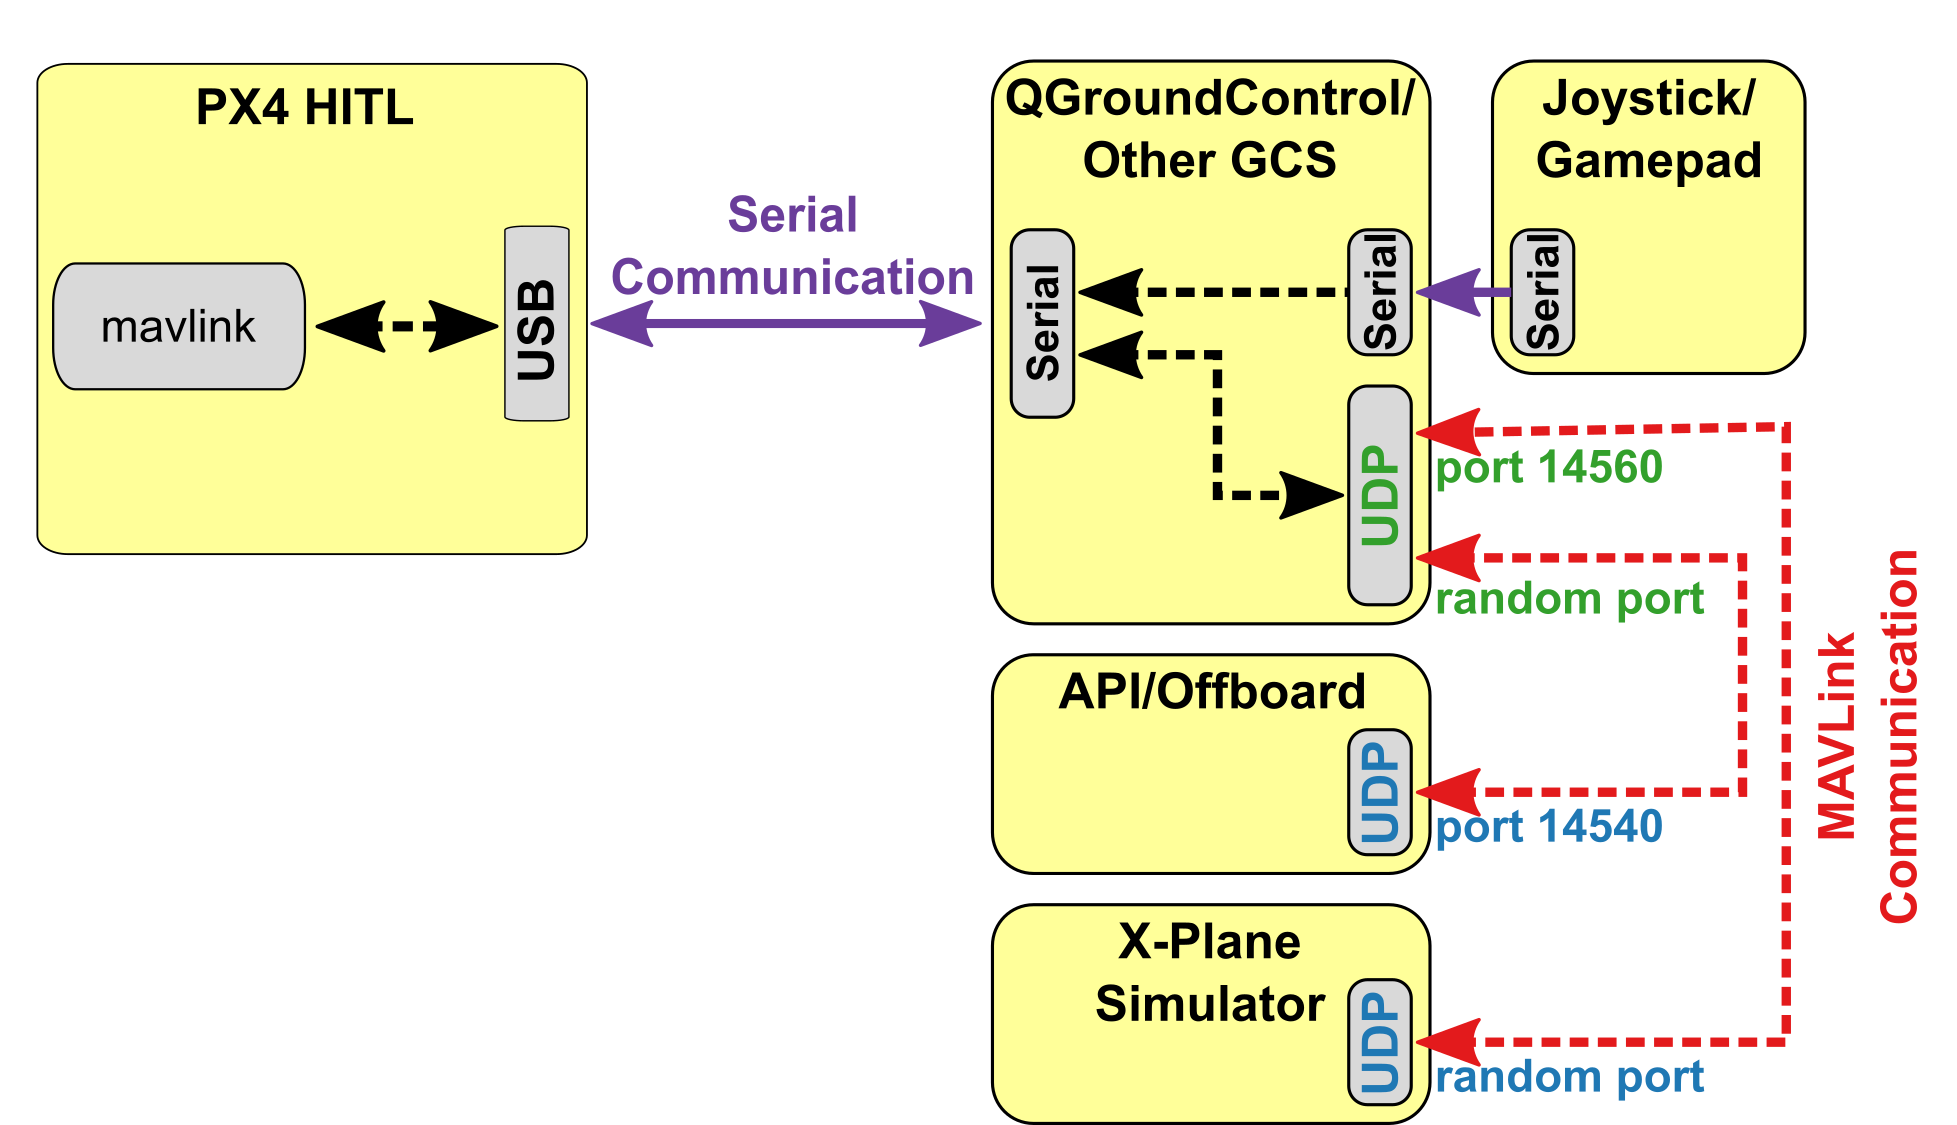
\includegraphics[width=0.8\textwidth]{picture/hitl.png}
    %   \caption{HITL-Xplane}
    % \end{figure}
    % \begin{figure}[htbp]
    %   \centering
    %   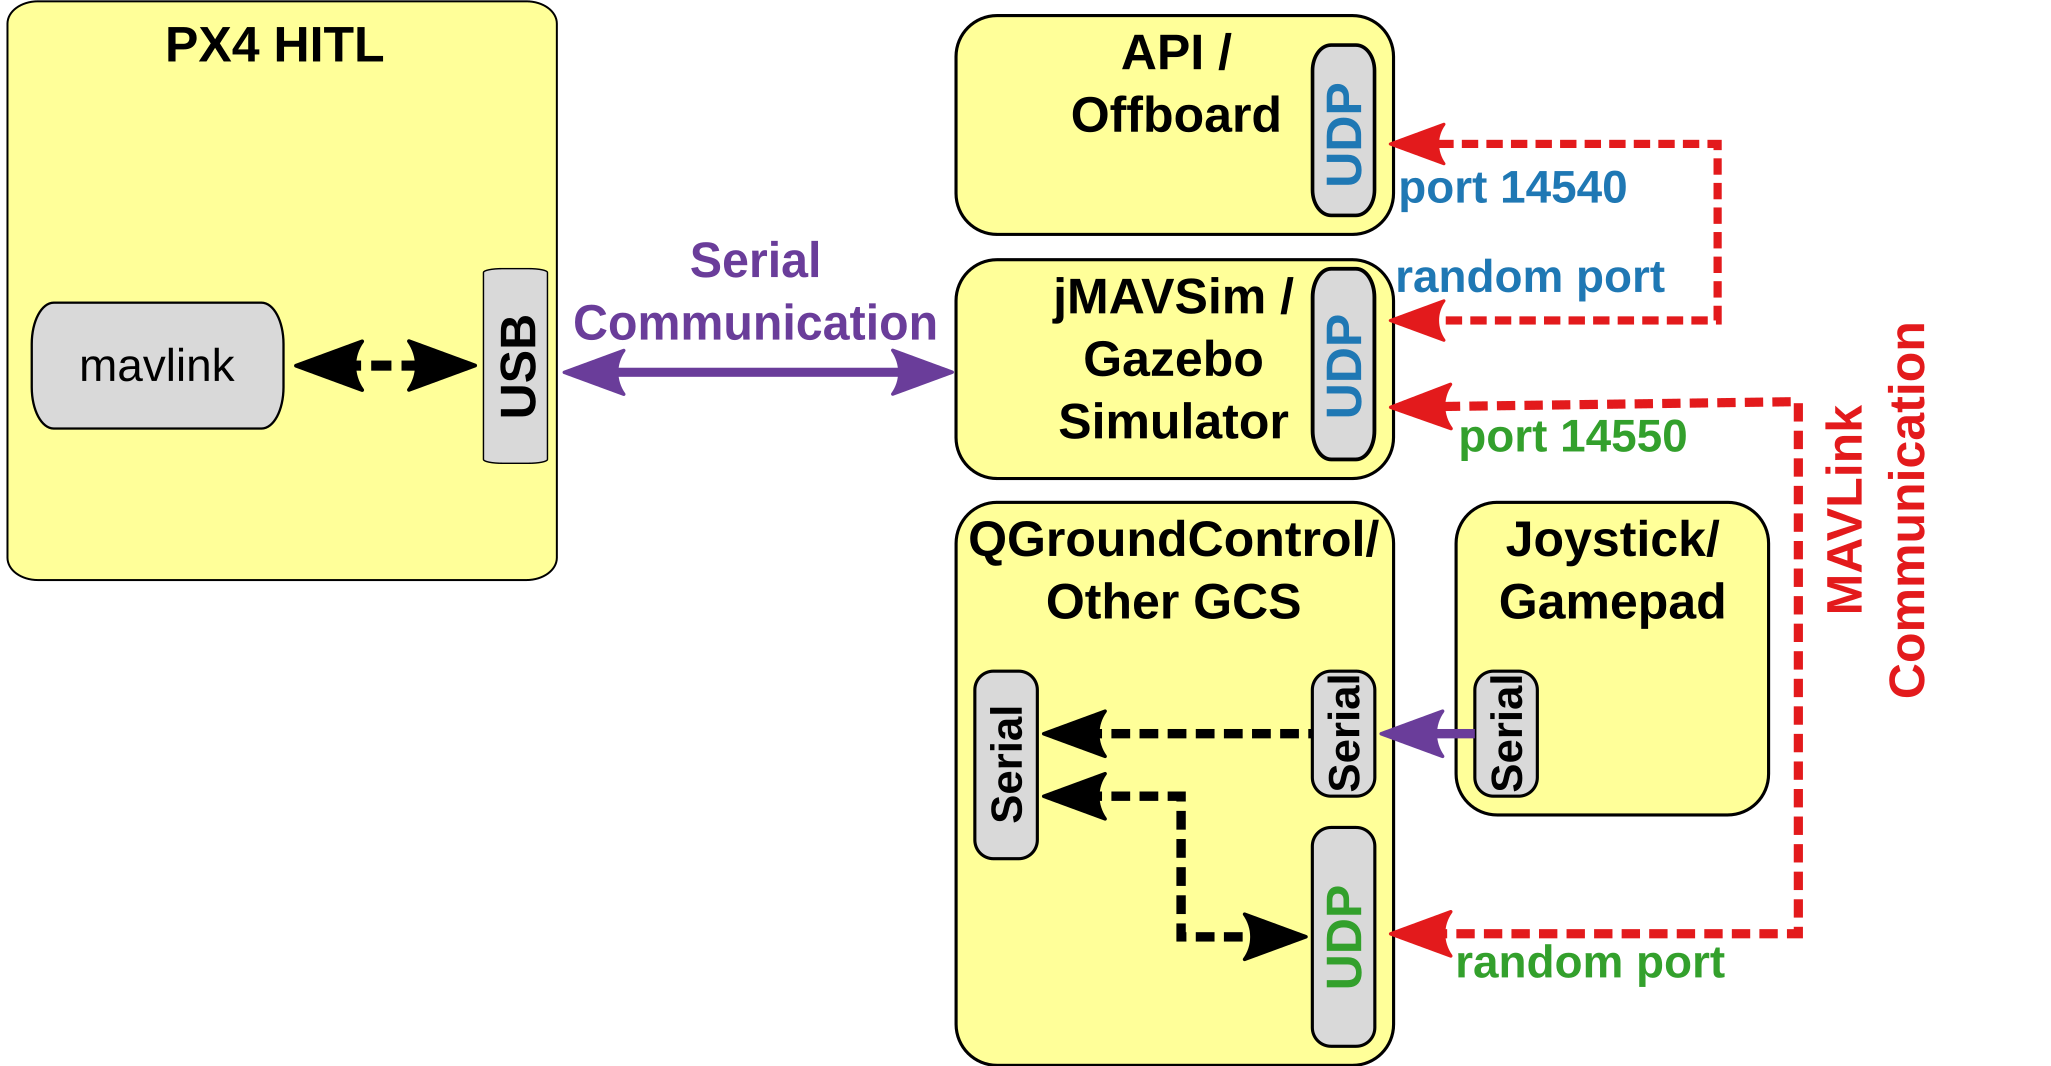
\includegraphics[width=0.8\textwidth]{picture/hitl2.png}
    %   \caption{HITL-Gazebo}
    % \end{figure}
    % \clearpage
    % \section{计算机视觉}
    %     整理一下当前的任务流.
    %   计算机视觉, 是一门研究如何对数字图像或视频进行高层语义理解的交叉学科, 赋予了机器"看"的能力, 需要实现人的大脑中(主要是视觉皮层区)的视觉能力. \par
    %   图像处理, 用计算机对图像进行分析, 已达到所需结果的技术. 图像处理一般指的是数字图像处理, 图像处理的技术一般包括图像压缩, 增强和复原, 匹配, 描述和识别三个部分. 
    %   \par 图像处理就是各种的图像变换处理, 计算机视觉在图像处理之后再识别其内部的语义, 理解视频流中的内容. 
    % \begin{figure}[htbp]
    %     \centering
    %     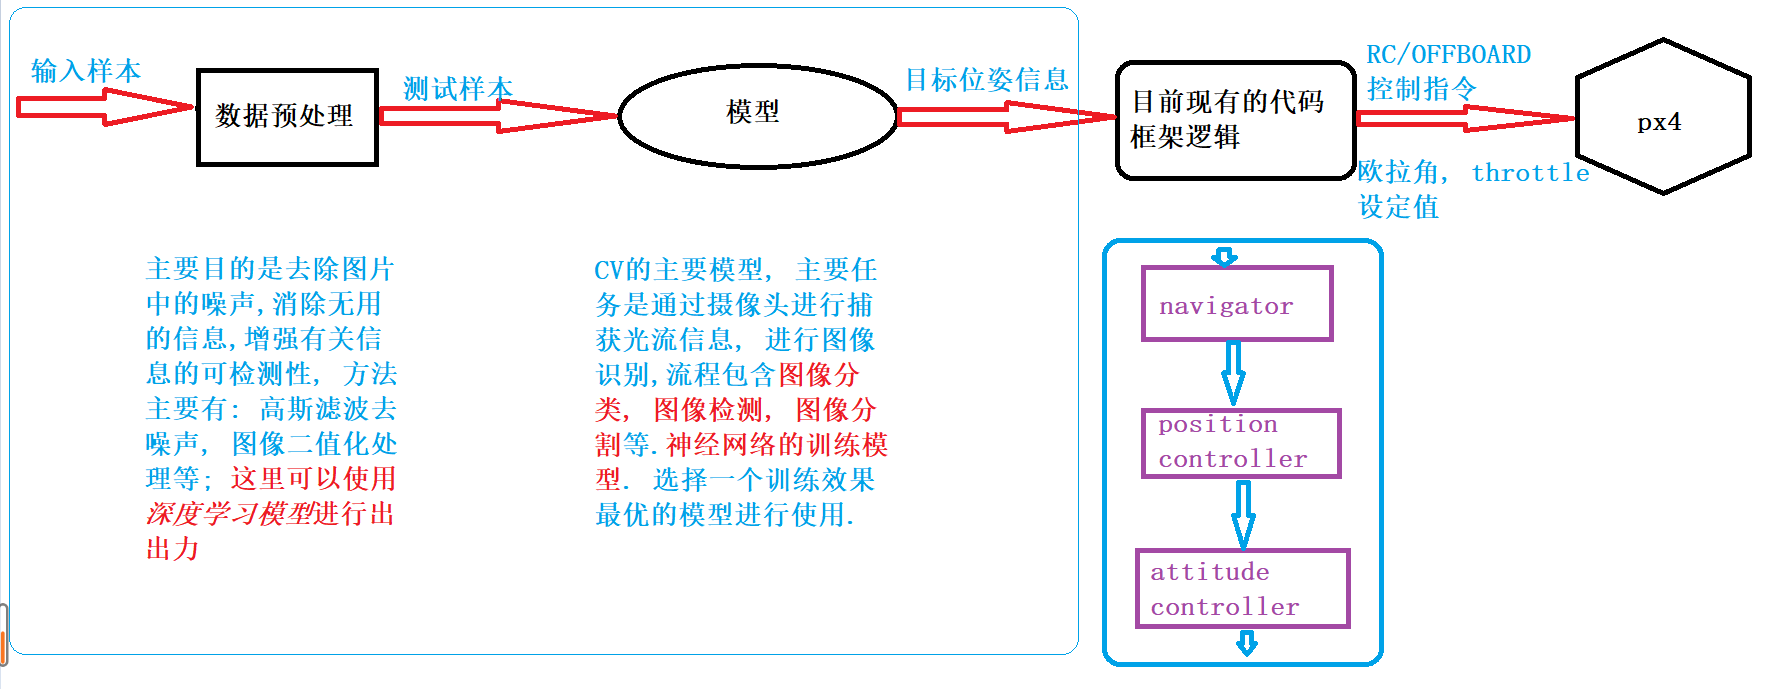
\includegraphics[width=0.8\textwidth]{picture/CV_Flow.png}
    %     \caption{CV数据流}
    % \end{figure}  
    % \clearpage
    % \section{算法内部}
    %     有时间的话细说一下代码
\end{document}
